%The paper size, font size and document type are defined in the following
\documentclass[a4paper,12pt]{article}

%Uncomment the following line, if you write in Finnish (special characters)
%\usepackage[utf8]{inputenc}

% Algorithm package
\usepackage[linesnumbered,ruled,vlined]{algorithm2e}
\renewcommand{\algorithmautorefname}{Algorithm}

%\usepackage[finnish]{babel}
\usepackage[english]{babel}

\usepackage{graphicx}
\usepackage[parfill]{parskip}

%useful special symbols:
\usepackage{amssymb}
\usepackage{latexsym}
\usepackage{amsmath}
\usepackage{amsthm}

\usepackage[toc,page]{appendix}

%a useful package if you write url addresses:
\usepackage{url}
\usepackage{hyperref}

%a package for figures:
% \usepackage[dvips]{color}
\usepackage{epsfig}

%a package for rotated figures and tables:
\usepackage{rotating}

\usepackage{biblatex}
\addbibresource{references.bib}

\usepackage{listings} % For including code
\usepackage{xcolor}   % For defining code colors

\usepackage{float}

%% Define custom colors for the code
\definecolor{codegreen}{rgb}{0,0.6,0}
\definecolor{codegray}{rgb}{0.5,0.5,0.5}
\definecolor{codepurple}{rgb}{0.58,0,0.82}
\definecolor{backcolour}{rgb}{0.95,0.95,0.92}

% Define Python code style
\lstdefinestyle{mystyle}{
    backgroundcolor=\color{backcolour},   
    commentstyle=\color{codegreen},
    keywordstyle=\color{magenta},
    numberstyle=\tiny\color{codegray},
    stringstyle=\color{codepurple},
    basicstyle=\ttfamily\footnotesize,
    breakatwhitespace=false,         
    breaklines=true,                 
    captionpos=b,                    
    keepspaces=true,                 
    numbers=left,                    
    numbersep=5pt,                  
    showspaces=false,                
    showstringspaces=false,
    showtabs=false,                  
    tabsize=4
}

% Apply the style to Python listings
\lstset{style=mystyle}

\graphicspath{ {./figures/} }

%if you want smaller page margins, uncomment and adjust the following
%\textheight=24.3cm
%\topmargin=-1.8cm
%\textwidth=16.7cm
%\oddsidemargin=-0.3cm
%\evensidemargin=0.0cm


%Create your own environments
\newtheorem{definition}{Definition}
\newtheorem{example}{Example}
\newtheorem{theorem}{Theorem}

%and useful macrosfor faster writing (benefit: you can change the notations 
%later, e.g., two possible notations for your vector x)
\newcommand{\Mmatr}{\ensuremath{\mathbf{M}}}
\newcommand{\xvec}{\ensuremath{\overline{x}}}
\newcommand{\xvecII}{\ensuremath{\mathbf{x}}} %alternative def
\newcommand{\Xset}{\ensuremath{\mathbf{X}}}
\newcommand{\fr}{\ensuremath{\mathit{fr}}} %just neater typing

%If you want to remove the space before paragraphs uncomment the following.
%Remember then to leave an empty line between paragraphs! 
%\setlength{\parindent}{0pt}


\title{MDM-2024 Homework 4}
\author{Cuong Nguyen (101559968), Petteri Raita (909635),\\and Raihan Gafur (101555441)}

%Uncomment the following, if you don't want the date to be printed
%\date{}

\begin{document}

\maketitle
\tableofcontents
\newpage

\listoffigures
\newpage

\section{Basic depth-first search}
% Briefly describe the algorithm
The algorithm is a basic depth-first search (DFS) algorithm that finds all cliques in a graph. The algorithm starts by iterating through all nodes in the graph and calling the DFS function on each node. The DFS function recursively explores the graph starting from the given node and adds nodes to the current clique if they satisfy a certain condition. The algorithm uses a helper function \texttt{shouldAddNode} to determine whether a node should be added to the current clique based on the \autoref{thm:pruning_theorem}. The algorithm returns a set of all cliques found in the graph.

To avoid adding duplicated cliques regardless the order of nodes in the clique, the algorithm uses a set data structure to store the cliques.

The Psuedocode for the algorithm is shown in \autoref{alg:basic-dfs}.


\SetKwComment{Comment}{/* }{ */}
\begin{algorithm}
    \caption{Basic depth-first search}
    \label{alg:basic-dfs}
    % \SetKwFunction{FMyFunction}{MyFunction}
    \SetKwProg{Fn}{Function}{:}{}

    \Fn{shouldAddNode($S$, $graph$, $node$, $\alpha$)}{
        $superS := S$ union $\{node\}$ \Comment*[r]{Set union operation}
        \For{$v$ in $S$}{
            \If{$ f(superS) < 1 - \frac{graph.degree(node) \times (1-\alpha)}{(|S| - 1)\times \alpha}$}{
                \KwRet{False}
            }
            \textbf{end if}
        }
        \textbf{end for}

        \KwRet{True}
    }

    \Fn{DFS($S$, $grah$, $startNode$, $visited$, $cliques$, $\alpha$)}{
        % Mark the current node as visited

        $visited.add(startNode)$ \Comment*[r]{Set data structure does not allow duplicates}
        \If{$f(S) \ge \alpha$}{
            $cliques.add(S)$\;
        }
        \textbf{end if}\

        \For{$v$ in $graph.neighbors(startNode)$}{
            \If{($v$ not in $visited$) and $shouldAddNode(S, graph, v, \alpha)$}{
                $newS := S$ union $\{v\}$ \Comment*[r]{Set union operation}
                $DFS(newS, graph, v, visited, cliques, alpha)$\;
            }
            \textbf{end if}
        }
        \textbf{end for}

        \KwRet
    }

    $G := (V,E)$ \Comment*[r]{Graph $G$ with vertices $V$ and edges $E$}
    $cliques := \emptyset$ \Comment*[r]{Set of cliques}
    \For{$root$ in $G.nodes$}{
        $visited := \emptyset$ \Comment*[r]{Set of visited nodes}
        $initialS := \{root\}$\;
        $DFS(initialS, G, root, \emptyset, cliques, \alpha)$\;
    }
    \textbf{end for}

    \KwRet{$cliques$}
\end{algorithm}
\section{Improved Algorithm}

The improved algorithm focuses on the selection of cliques based on the smallest degree nodes and uses a theorem to prune the search space efficiently.
The primary improvement lies in selecting cliques starting with nodes that have the smallest degree, \( \deg(v) \), in the entire graph.

\begin{theorem}
    \label{thm:pruning_theorem} % Label for referencing
    If
    \[
        f(S) < 1 - \frac{\deg(v) (1 - \alpha)}{(|S| - 1) \alpha}
    \]
    for any \( v \in S \), then none of \( S \)'s supersets can be an \( \alpha \)-clique.
\end{theorem}

\paragraph{Pruning Mechanism Using Theorem}
The pruning mechanism is governed by the ~\autoref{thm:pruning_theorem} that sets a condition on when a set \( S \) and its supersets can be classified as non-\( \alpha \)-cliques. For effective pruning:
\begin{itemize}
    \item The condition must hold more frequently.
    \item The upper bound on the right-hand side (RHS) of the theorem must be maximized.
\end{itemize}
Maximizing the RHS upper bound involves minimizing the negative term associated with \( \deg(v) \). Therefore, iterating over nodes from the smallest to largest degree makes the pruning happen as often as possible.

\paragraph{Illustration}
A visual representation of the improvement is shown in  ~\autoref{fig:improved_algorithm}. In the graph, the differing values tested candidates per  \(\alpha\), show the computation performance of the improved algorithm. For smaller  \(\alpha\) values, the effect is more pronounced, but even for the  \(\alpha = 0.8\) , the improved algorithm does 47 comparisons less. With  \(\alpha\) reaching 1, there is no difference with the improved and traditional algorithm. This happens, since the RHS of the theorem will become always 1. The exact values of \(\alpha\) are show in ~\autoref{tab:tested_candidates}

\begin{table}[h]
    \centering
    \begin{tabular}{ccc}
        \hline
        \(\alpha\) & Basic Algorithm & Improved Algorithm \\
        \hline
        0.5        & 1613            & 1471               \\
        0.6        & 1261            & 1127               \\
        0.7        & 1006            & 902                \\
        0.8        & 621             & 574                \\
        \hline
    \end{tabular}
    \caption{Exact values of tested candidates per  \(\alpha\)}
    \label{tab:tested_candidates} % Added label for referencing
\end{table}


\paragraph{Impact of Graph Size on \(\alpha\)}
For future research, the effect of the size of the graph for pruning could be studied. The size might affect the number of candidates tested that the pruning affects. Possbily in larger graphs, the impact of the improved pruning algorithm might save more tested candidates.

\begin{figure}[h]
    \centering
    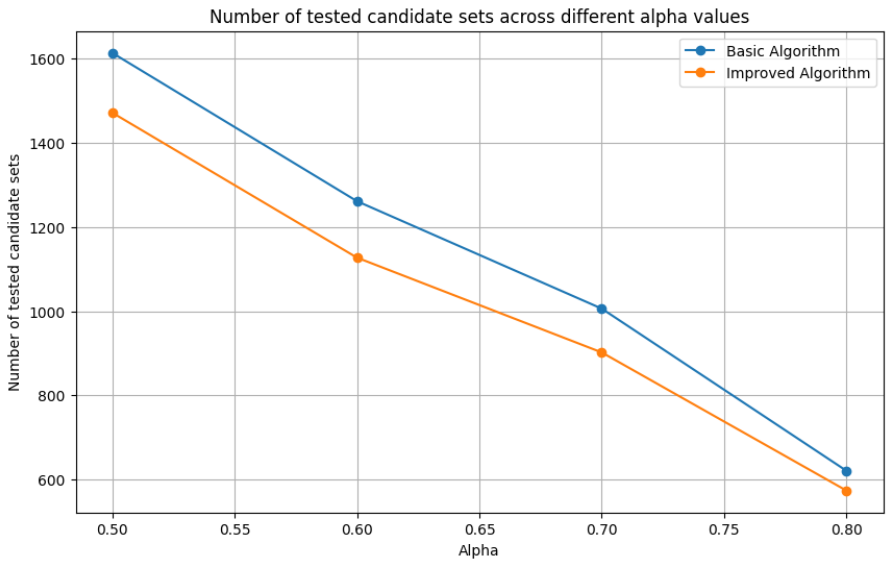
\includegraphics[width=0.8\textwidth]
    {figures/improved_algorithm.png}
    \caption{Number of tested candidates per \(\alpha\)}
    \label{fig:improved_algorithm}
\end{figure}

\section{Experiments in the dolphin data}
This study investigated maximal alpha-cliques within a dolphin social network data using an alpha threshold of 0.8, with cliques comprising at least five dolphins. The analysis identified four maximal cliques, each reflecting unique gender distributions, providing insights into potential social dynamics influenced by gender within the dolphin community.

\subsection{Maximal Alpha-Clique 1}
\textbf{Composition}: Jonah, MN105, MN83, Patchback, Topless, and Trigger. \\
\textbf{Gender Distribution}: This clique predominantly consists of males, with five males and one female. \\
\textbf{Interpretation}: The male dominance within this group suggests that male dolphins in this network may form strong social bonds with limited female presence. Such a configuration could indicate either a preference for male companionship or shared behaviors and social interactions unique to male dolphins within this subset of the network.
\begin{figure}[H]
    \centering
    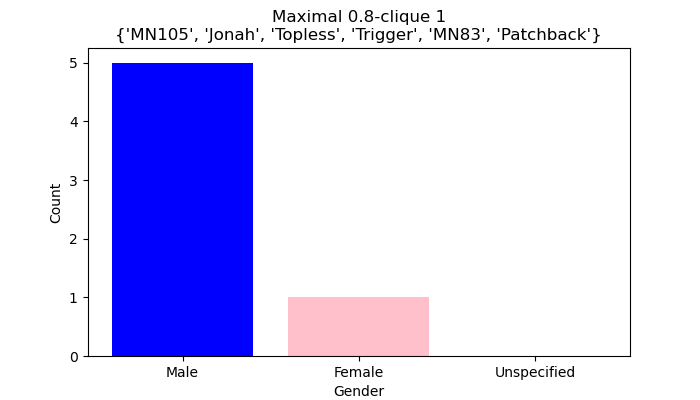
\includegraphics[width=1.0\textwidth]{clique_1.png}
    \caption{Clique 1}
    \label{fig:clique_1}
\end{figure}

\subsection{Maximal Alpha-Clique 2}
\textbf{Composition}: Grin, Hook, SN4, SN63, Scabs, and Stripes. \\
\textbf{Gender Distribution}: All members in this clique are female. \\
\textbf{Interpretation}: The exclusivity of female members in this clique suggests a gender-based social structure, where female dolphins are inclined to form tightly-knit groups. This homogeneous grouping may reflect social bonding patterns or cooperative behaviors specific to females, potentially serving as mechanisms for support or protection within the dolphin community.
\begin{figure}[H]
    \centering
    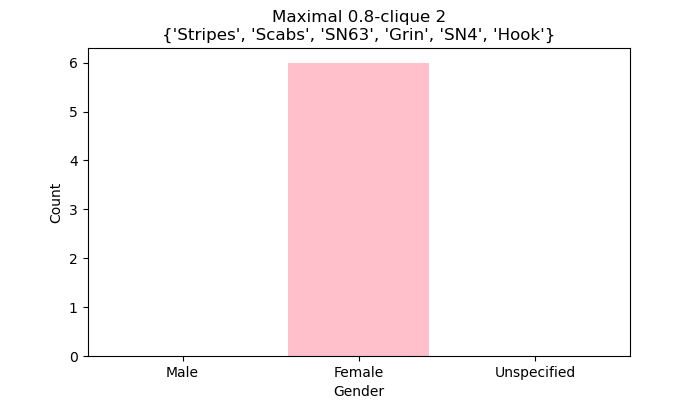
\includegraphics[width=1.0\textwidth]{clique_2.png}
    \caption{Clique 2}
    \label{fig:clique_2}
\end{figure}

\subsection{Maximal Alpha-Clique 3}
\textbf{Composition}: DN21, Feather, Gallatin, SN90, Upbang, and Web. \\
\textbf{Gender Distribution}: This clique is exclusively male. \\
\textbf{Interpretation}: The existence of a male-only clique, similar to Clique 1 but with a complete absence of females, highlights a pattern of strong male alliances. The homogeneous nature of this clique may suggest a stable network of male friendships or alliances that play a role in male social strategies, possibly for cooperation in social or territorial behaviors within their community.
\begin{figure}[H]
    \centering
    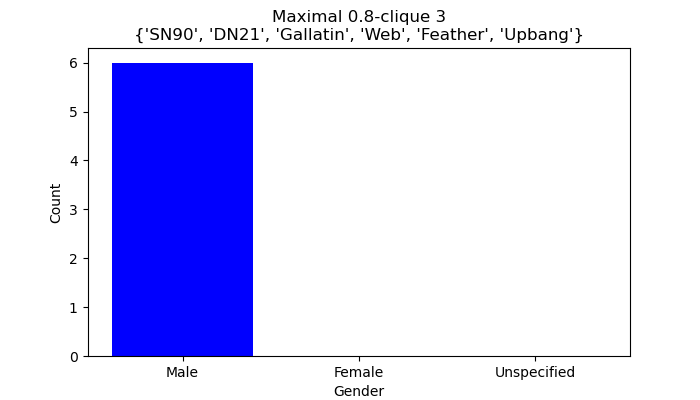
\includegraphics[width=1.0\textwidth]{clique_3.png}
    \caption{Clique 3}
    \label{fig:clique_3}
\end{figure}

\subsection{Maximal Alpha-Clique 4}
\textbf{Composition}: DN21, Feather, Gallatin, Jet, and Web. \\
\textbf{Gender Distribution}: Like Clique 3, this group is exclusively male. \\
\textbf{Interpretation}: This smaller, all-male clique demonstrates a tightly interconnected subgroup, as indicated by its higher internal connectivity (fs = 1.00). This high level of connectivity suggests an exceptionally stable social structure within the male subgroup, reinforcing the hypothesis that male dolphins form strong, exclusive bonds that could serve social or survival functions within the community.
\begin{figure}[H]
    \centering
    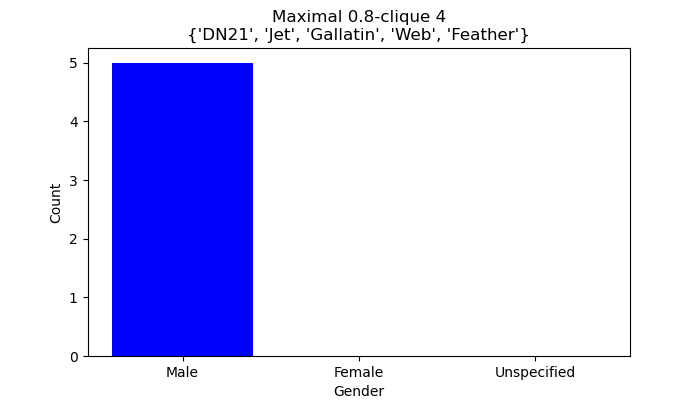
\includegraphics[width=1.0\textwidth]{clique_4.png}
    \caption{Clique 4}
    \label{fig:clique_4}
\end{figure}

The observed gender distributions within the maximal alpha-cliques reveal notable patterns of gender-based social structuring in the dolphin community. Specifically, cliques tend to exhibit gender homogeneity, with all-female or all-male groups forming more frequently than mixed-gender groups. This tendency suggests that gender plays a significant role in the formation and cohesion of social subgroups within the dolphin network, potentially influenced by behaviors, social preferences, or survival strategies specific to each gender.

In conclusion, this analysis underscores the complexity of dolphin social behavior, emphasizing the influence of gender on subgroup formation within their networks. Based on the assumption that the graph is naturally connected, it would be interesting to run the analysis on a more accurate weighted graph to see the difference between an unweighted and a weighted graph. Intuitively, the weighted graph would produce a more accurate clustering. Additionally, a comparison to the clustering of other sea mammals would produce better interpretation of the result.
% include tex files of sections here, e.g.
% \input{section1.tex}
% \input{section2.tex}


%Bibliography style. The alpha style generates references with 
%first letters and year. If you prefer numbers, use style plain.
% \bibliographystyle{alpha}
% \bibliographystyle{plain}
% \bibliography{ref}

% \printbibliography{}

% Demo for adding appendices
% \begin{appendices}
%     All code is publicly available on GitHub at \url{https://github.com/ancuongnguyen07/CS-E4650/tree/master/hw5}
% \end{appendices}


\end{document}
